%!TEX root = ../../../main.tex
%%---------------------------------------------------------------------------
\section{Work-cell modelling and calibration}
\label{sec:workcell}
%%---------------------------------------------------------------------------
Due to new robots and new work-cells a complete new modelling of the work-cell was needed. Since RobWork and RobWorkStudio was used, the format was given by these frameworks. 

The modelling of the Kuka Kr6 robot was done by converting an existing 3D model and creating the corresponding XML files. The conveyor belt was measured and designed in a CAD program. The gripper model was and the rest of the cell elements was copied from another similar work-cell used in earlier projects. 

The calibration of the scene elements was done in two steps. A rough calibration was done based on physical measurements. The more precise calibration consisted of jogging the robot to different points in the scene and measuring the difference in the scene compared to the difference in the real world, minimizing this error during a few iterations. \\

Figure \ref{fig:rc_frames} shows a section from the scene. The TCP frame of the gripper is shown alongside the frame in which the collected Lego bricks is delivered at and the defined center frame of the conveyor belt. All Lego bricks are defined in this frame. The frame of the camera mounted the gripper is shown as well. 

	\begin{figure}[H]
		\centering
	    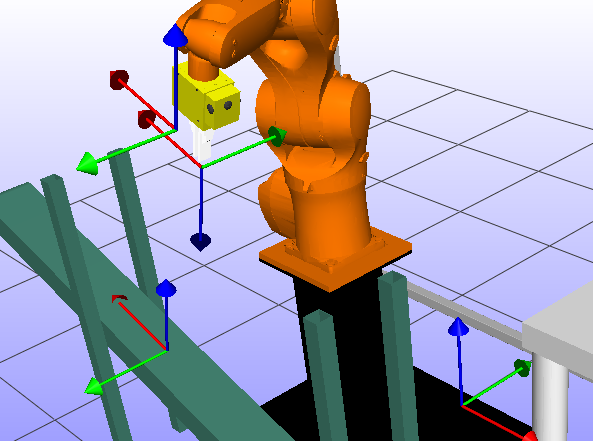
\includegraphics[width=0.7\textwidth]{rc_frames}
	    \caption{Work-cell: Gripper, camera, conveyor-belt and delivery frame}
		\label{fig:rc_frames}
	\end{figure}
	
Lastly the calibration between the gripper, conveyor and camera was archived using a simple yet effective method. The center of the conveyor frame was marked on the real conveyor by aligning the z-axis of the gripper and conveyor frame, making the gripper fingers point at this center point. Next the center of the camera and conveyor frame was aligned and the marked point should now be at the center of the image as well. By looking at the offset and correcting the required amount, this method proved good.  